
\begin{figure}[h!]
	\centering
	\tikzset{every picture/.style={line width=0.75pt}} %set default line width to 0.75pt        
	
	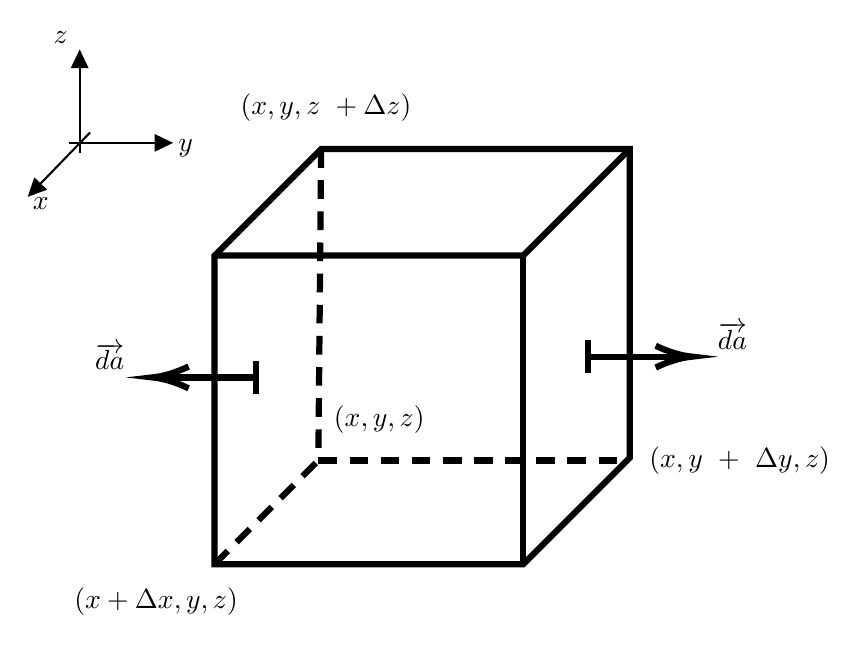
\begin{tikzpicture}[x=0.75pt,y=0.75pt,yscale=-1,xscale=1]
		%uncomment if require: \path (0,300); %set diagram left start at 0, and has height of 300
		
		%Shape: Cube [id:dp6052690098400888] 
		\draw  [line width=2.25]  (200,101.31) -- (251.31,50) -- (400,50) -- (400,198.69) -- (348.69,250) -- (200,250) -- cycle ; \draw  [line width=2.25]  (400,50) -- (348.69,101.31) -- (200,101.31) ; \draw  [line width=2.25]  (348.69,101.31) -- (348.69,250) ;
		%Straight Lines [id:da6838346844891714] 
		\draw [line width=2.25]  [dash pattern={on 6.75pt off 4.5pt}]  (250,200) -- (400,200) ;
		%Straight Lines [id:da4358863669422177] 
		\draw [line width=2.25]  [dash pattern={on 6.75pt off 4.5pt}]  (251.31,50) -- (250,200) ;
		%Straight Lines [id:da8699451449684632] 
		\draw [line width=2.25]  [dash pattern={on 6.75pt off 4.5pt}]  (200,250) -- (250,200) ;
		%Straight Lines [id:da6153923820857115] 
		\draw [line width=2.25]    (220,160) -- (174,160) ;
		\draw [shift={(170,160)}, rotate = 360] [color={rgb, 255:red, 0; green, 0; blue, 0 }  ][line width=2.25]    (17.49,-5.26) .. controls (11.12,-2.23) and (5.29,-0.48) .. (0,0) .. controls (5.29,0.48) and (11.12,2.23) .. (17.49,5.26)   ;
		\draw [shift={(220,160)}, rotate = 360] [color={rgb, 255:red, 0; green, 0; blue, 0 }  ][line width=2.25]    (0,7.83) -- (0,-7.83)   ;
		%Straight Lines [id:da3502060568264709] 
		\draw [line width=2.25]    (380,150) -- (426,150) ;
		\draw [shift={(430,150)}, rotate = 180] [color={rgb, 255:red, 0; green, 0; blue, 0 }  ][line width=2.25]    (17.49,-5.26) .. controls (11.12,-2.23) and (5.29,-0.48) .. (0,0) .. controls (5.29,0.48) and (11.12,2.23) .. (17.49,5.26)   ;
		\draw [shift={(380,150)}, rotate = 180] [color={rgb, 255:red, 0; green, 0; blue, 0 }  ][line width=2.25]    (0,7.83) -- (0,-7.83)   ;
		%Straight Lines [id:da8422422028495438] 
		\draw [line width=0.75]    (140,42) -- (112.09,70.84) ;
		\draw [shift={(110,73)}, rotate = 314.06] [fill={rgb, 255:red, 0; green, 0; blue, 0 }  ][line width=0.08]  [draw opacity=0] (8.93,-4.29) -- (0,0) -- (8.93,4.29) -- cycle    ;
		%Straight Lines [id:da7449366310627421] 
		\draw [line width=0.75]    (135,52) -- (135,5) ;
		\draw [shift={(135,2)}, rotate = 90] [fill={rgb, 255:red, 0; green, 0; blue, 0 }  ][line width=0.08]  [draw opacity=0] (8.93,-4.29) -- (0,0) -- (8.93,4.29) -- cycle    ;
		%Straight Lines [id:da9487980467676893] 
		\draw [line width=0.75]    (130,47) -- (177,47) ;
		\draw [shift={(180,47)}, rotate = 180] [fill={rgb, 255:red, 0; green, 0; blue, 0 }  ][line width=0.08]  [draw opacity=0] (8.93,-4.29) -- (0,0) -- (8.93,4.29) -- cycle    ;
		
		% Text Node
		\draw (256,172) node [anchor=north west][inner sep=0.75pt]   [align=left] {$\displaystyle ( x,y,z)$};
		% Text Node
		\draw (131,260) node [anchor=north west][inner sep=0.75pt]   [align=left] {$\displaystyle ( x+\Delta x,y,z)$};
		% Text Node
		\draw (408,192) node [anchor=north west][inner sep=0.75pt]   [align=left] {$\displaystyle ( x,y\ +\ \Delta y,z)$};
		% Text Node
		\draw (211,22) node [anchor=north west][inner sep=0.75pt]   [align=left] {$\displaystyle ( x,y,z\ +\Delta z)$};
		% Text Node
		\draw (111,72) node [anchor=north west][inner sep=0.75pt]   [align=left] {$\displaystyle x$};
		% Text Node
		\draw (181,44) node [anchor=north west][inner sep=0.75pt]   [align=left] {$\displaystyle y$};
		% Text Node
		\draw (121,-8) node [anchor=north west][inner sep=0.75pt]   [align=left] {$\displaystyle z$};
		% Text Node
		\draw (141,142) node [anchor=north west][inner sep=0.75pt]   [align=left] {$\displaystyle \overrightarrow{da}$};
		% Text Node
		\draw (441,132) node [anchor=north west][inner sep=0.75pt]   [align=left] {$\displaystyle \overrightarrow{da}$};
		
		
	\end{tikzpicture}
	\caption{The infinitesimal cube for deriving the continuity equation}
	\label{fig:infbox}
\end{figure}
